\documentclass[11pt]{article}
\usepackage{times}
\usepackage[cm]{fullpage}
\usepackage{amsmath,amssymb}
\usepackage{booktabs}
\usepackage{tabularx}
\newcolumntype{Y}{>{\raggedright\arraybackslash}X}
\usepackage{enumitem}
\usepackage{xcolor}
\usepackage{hyperref}
\usepackage{microtype}
\usepackage{tikz}
\usetikzlibrary{arrows.meta,positioning,fit,backgrounds,calc,shapes.geometric}
\hypersetup{hidelinks}

\definecolor{primitivecol}{RGB}{85,85,85}
\definecolor{optioncol}{RGB}{183,83,42}
\definecolor{landmarkcol}{RGB}{42,104,155}
\definecolor{goalcol}{RGB}{34,120,52}
\definecolor{mapcol}{RGB}{112,73,150}

\tikzset{
  arrow/.style={-{Stealth[length=4pt]},line width=0.85pt},
  biarrow/.style={{Stealth[length=3pt]}-{Stealth[length=3pt]},line width=0.8pt},
  stage/.style={draw,rounded corners=2pt,minimum width=22mm,minimum height=10mm,
    align=center,font=\small,fill=black!3},
  state/.style={circle,draw=primitivecol,minimum size=7mm,inner sep=0pt,font=\scriptsize},
  landmark/.style={circle,draw=landmarkcol,fill=landmarkcol!18,minimum size=8mm,
    inner sep=0pt,font=\scriptsize\bfseries},
  goal/.style={circle,draw=goalcol,fill=goalcol!15,minimum size=8mm,
    inner sep=0pt,font=\scriptsize\bfseries},
  dbn/.style={circle,draw,minimum size=9mm,inner sep=0pt,font=\small},
  panel/.style={draw=black!30,rounded corners=2pt,inner sep=5pt}
}

\title{How to Abstract a Problem-Solving Task?\\
\large Analysis 7: Probabilistic Cognitive Maps and Shared A$^\ast$ Planning}
\author{}
\date{12 June 2026}

\begin{document}
\maketitle

\begin{abstract}
This note defines the representation and planning algorithm for three agent families:
a primitive planner, an action-chunk planner, and a landmark planner. Each representation
induces a row-stochastic transition kernel $P_M(v'\mid v)$. Transition probabilities become
additive surprisal costs, directed shortest-path costs define cognitive geodesics, and a
two-dimensional Isomap/classical-MDS embedding provides a geometric cognitive map. All
families then use the same A$^\ast$ algorithm with an embedding-based heuristic scaled to
be consistent and admissible. The landmark family is a two-slice dynamic Bayesian network
with a landmark core and a non-landmark periphery: landmark-to-landmark,
landmark-to-non-landmark, and non-landmark-to-landmark probabilities are represented
explicitly, whereas direct non-landmark-to-non-landmark transitions are absent. This note
does not define trajectory segmentation, behavioral emissions, or representation recovery;
those are inference questions delegated to Analysis 8.
\end{abstract}

\section{Scope and common architecture}

Let $\mathcal S$ be the primitive state space and let
\[
\mathcal M
=
\{M_{\mathrm{primitive}},M_{\mathrm{option}},M_{\mathrm{landmark}}\}
\]
be the three candidate agent families. Analysis 7 is concerned only with the agent's
stored representation and the planning computation that follows from it:
\begin{equation}
\boxed{
\mathcal R_M
\longrightarrow
P_M(v'\mid v)
\longrightarrow
c_M
\longrightarrow
d_M^\to
\longrightarrow
\psi_M
\longrightarrow
\mathrm{A}^{\ast}.
}
\label{eq:architecture}
\end{equation}
The induced probabilistic cognitive transition structure is
\begin{equation}
\mathcal K_M
=
F_M(\mathcal K_0,\mathcal R_M)
=
(\mathcal V_M,P_M),
\qquad
\sum_{v'\in\mathcal V_M}P_M(v'\mid v)=1.
\label{eq:map}
\end{equation}
For the present task $\mathcal V_M=\mathcal S$ for all families. The families differ in
how they construct $P_M$, but probability-to-distance conversion, manifold learning, and
A$^\ast$ search are identical.

\begin{table}[htbp]
\centering
\small
\begin{tabularx}{\textwidth}{lYY}
\toprule
Family & Stored representation $\mathcal R_M$ & Induced transition kernel \\
\midrule
Primitive & Primitive action probabilities & State transitions obtained from
length-one action tokens \\
Action chunk & Grammar $\mathcal G$ and executable-token probabilities
$q_{\mathcal G}(g\mid x)$ & State transitions marginalized over primitive and chunk
tokens with the same endpoint \\
Landmark & Landmark set $\mathcal L$ and three CPD blocks
$p(\ell'\mid\ell)$, $p(u\mid\ell)$, $p(\ell\mid u)$ &
Core--periphery transition PGM with no direct $u\to u'$ edge \\
\bottomrule
\end{tabularx}
\caption{The three representations differ before the shared probability-geometry-planning
pipeline. Here and below $u,u'\in\mathcal U:=\mathcal S\setminus\mathcal L$ denote
non-landmarks.}
\label{tab:families}
\end{table}

\section{The landmark representation is a transition PGM}
\label{sec:landmark}

Let $\mathcal L\subset\mathcal S$ be the landmark set and
$\mathcal U=\mathcal S\setminus\mathcal L$ the non-landmarks. The landmark agent stores
one conditional transition distribution
\begin{equation}
P_{\mathrm L}(v'\mid v)
=
\begin{cases}
p(\ell'\mid\ell),
& v=\ell,\ v'=\ell',\\
p(u\mid\ell),
& v=\ell,\ v'=u,\\
p(\ell\mid u),
& v=u,\ v'=\ell,\\
0,
& v=u,\ v'=u'.
\end{cases}
\label{eq:landmark-kernel}
\end{equation}
The probabilities in each source row are normalized \emph{jointly}. Thus
\begin{align}
\sum_{\ell'\in\mathcal L}p(\ell'\mid\ell)
+\sum_{u\in\mathcal U}p(u\mid\ell)&=1
\quad &&\text{for every }\ell\in\mathcal L,
\label{eq:row-landmark}\\
\sum_{\ell\in\mathcal L}p(\ell\mid u)&=1
\quad &&\text{for every }u\in\mathcal U.
\label{eq:row-nonlandmark}
\end{align}
Ordering states as $(\mathcal L,\mathcal U)$ gives the block transition matrix
\begin{equation}
P_{\mathrm L}
=
\begin{bmatrix}
P_{\mathcal L\mathcal L} & P_{\mathcal L\mathcal U}\\
P_{\mathcal U\mathcal L} & \mathbf 0
\end{bmatrix}.
\label{eq:block-matrix}
\end{equation}
Equation~\eqref{eq:landmark-kernel} is a two-slice dynamic Bayesian network, or
equivalently a first-order Markov transition PGM. Its unrolled graph is acyclic in time,
although the state-transition graph represented by $P_{\mathrm L}$ may contain directed
cycles. It should therefore not be described as one static Bayesian-network DAG over the
state labels.

\begin{figure}[htbp]
\centering
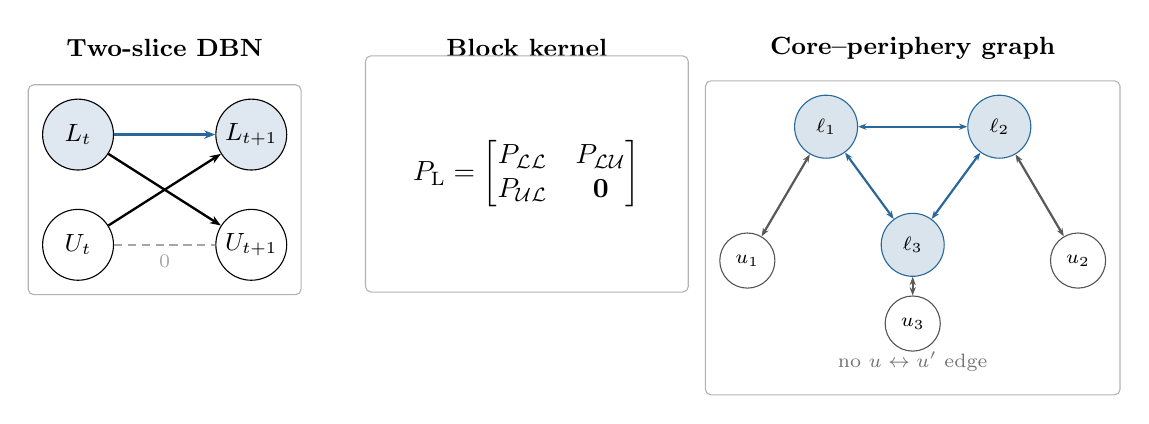
\begin{tikzpicture}[x=1cm,y=1cm]
  % DBN panel
  \node[font=\bfseries\small] at (1.8,2.8) {Two-slice DBN};
  \node[dbn,fill=landmarkcol!15] (Lt) at (0.7,1.7) {$L_t$};
  \node[dbn] (Ut) at (0.7,0.3) {$U_t$};
  \node[dbn,fill=landmarkcol!15] (Ln) at (2.9,1.7) {$L_{t+1}$};
  \node[dbn] (Un) at (2.9,0.3) {$U_{t+1}$};
  \draw[arrow,landmarkcol] (Lt)--(Ln);
  \draw[arrow] (Lt)--(Un);
  \draw[arrow] (Ut)--(Ln);
  \draw[densely dashed,black!35,line width=0.8pt] (Ut)--(Un)
    node[midway,below,sloped,font=\scriptsize] {$0$};
  \node[panel,fit=(Lt)(Ut)(Ln)(Un)] {};

  % matrix panel
  \node[font=\bfseries\small] at (6.4,2.8) {Block kernel};
  \node at (6.4,1.2) {$\displaystyle
    P_{\mathrm L}=
    \begin{bmatrix}
      P_{\mathcal L\mathcal L} & P_{\mathcal L\mathcal U}\\
      P_{\mathcal U\mathcal L} & \mathbf 0
    \end{bmatrix}$};
  \node[panel,minimum width=4.1cm,minimum height=3.0cm] at (6.4,1.2) {};

  % core-periphery panel
  \node[font=\bfseries\small] at (11.3,2.8) {Core--periphery graph};
  \node[landmark] (l1) at (10.2,1.8) {$\ell_1$};
  \node[landmark] (l2) at (12.4,1.8) {$\ell_2$};
  \node[landmark] (l3) at (11.3,0.3) {$\ell_3$};
  \draw[biarrow,landmarkcol] (l1)--(l2);
  \draw[biarrow,landmarkcol] (l1)--(l3);
  \draw[biarrow,landmarkcol] (l2)--(l3);
  \node[state] (u1) at (9.2,0.1) {$u_1$};
  \node[state] (u2) at (13.4,0.1) {$u_2$};
  \node[state] (u3) at (11.3,-0.7) {$u_3$};
  \draw[biarrow,black!65] (u1)--(l1);
  \draw[biarrow,black!65] (u2)--(l2);
  \draw[biarrow,black!65] (u3)--(l3);
  \node[font=\scriptsize,black!55] (noUU) at (11.3,-1.18)
    {no $u\leftrightarrow u'$ edge};
  \node[panel,fit=(l1)(l2)(l3)(u1)(u2)(u3)(noUU)] {};
\end{tikzpicture}
\caption{The landmark representation. Left: the allowed dependencies in one transition
of the two-slice DBN. Middle: the equivalent block transition matrix. Right: landmarks
form a mutually connected core; non-landmarks can enter or leave that core but cannot
transition directly to another non-landmark. The right panel is schematic rather than an
embedding.}
\label{fig:landmark-pgm}
\end{figure}

\subsection{The landmark core is a probability constraint}

The zero block $P_{\mathcal U\mathcal U}=\mathbf 0$ ensures that every plan from one
non-landmark to another must enter the landmark layer. To make the landmark layer a
\emph{tight} core in probability geometry, direct core transitions also satisfy, for
distinct $\ell,\ell'\in\mathcal L$,
\begin{equation}
p(\ell'\mid\ell)>0,
\qquad
p(\ell'\mid\ell)
\ge
\max_{u\in\mathcal U}
p(u\mid\ell)\,p(\ell'\mid u).
\label{eq:core-constraint}
\end{equation}
The right-hand side is the probability of the best two-edge detour
$\ell\to u\to\ell'$. Because surprisal is negative log probability,
\eqref{eq:core-constraint} implies
\[
-\log p(\ell'\mid\ell)
\le
-\log p(u\mid\ell)-\log p(\ell'\mid u).
\]
Any path that repeatedly leaves and re-enters the landmark layer can therefore be replaced,
one peripheral excursion at a time, by a path that remains in the landmark core with no
greater cost. The constraint makes core routes geodesically privileged over peripheral
detours. Absolute compactness is controlled by the magnitude of
$p(\ell'\mid\ell)$; the worked example makes this magnitude explicit rather than asking
the embedding algorithm to invent closeness.

\section{Primitive actions and action chunks induce the same object}
\label{sec:chunks}

Let $\mathcal T_{\mathcal G}(x)$ be the executable tokens at state $x$. It contains every
primitive action as a length-one production and, for the option family, every executable
chunk $g\in\mathcal G(x)$. The grammar supplies a normalized token distribution
\begin{equation}
\sum_{g\in\mathcal T_{\mathcal G}(x)}
q_{\mathcal G}(g\mid x)=1.
\label{eq:grammar-normalization}
\end{equation}
If $f(x,g)$ is the endpoint reached by executing token $g$ from $x$, then the induced
state-transition kernel is
\begin{equation}
P_{\mathcal G}(x'\mid x)
=
\sum_{\substack{g\in\mathcal T_{\mathcal G}(x):\\ f(x,g)=x'}}
q_{\mathcal G}(g\mid x).
\label{eq:chunk-kernel}
\end{equation}
Marginalizing over tokens that share an endpoint makes
$P_{\mathcal G}(\cdot\mid x)$ row-stochastic. The primitive family is the special case in
which $\mathcal T_{\mathcal G}(x)$ contains only length-one actions. Thus grammar
probabilities and landmark CPDs are different representational hypotheses that induce the
same mathematical planning interface: a directed transition kernel $P_M$.

\section{From transition probability to cognitive geometry}
\label{sec:geometry}

Define the supported directed edges
\[
\mathcal E_M
=
\{(u,v)\in\mathcal V_M^2:P_M(v\mid u)>0\}.
\]
Each supported edge receives surprisal cost
\begin{equation}
c_M(u,v)
=
-\log P_M(v\mid u),
\qquad
c_M(u,v)=\infty
\ \text{if }P_M(v\mid u)=0.
\label{eq:surprisal}
\end{equation}
For a directed path $\pi=(v_0,\ldots,v_k)$,
\[
\sum_{r=0}^{k-1}c_M(v_r,v_{r+1})
=
-\log\prod_{r=0}^{k-1}P_M(v_{r+1}\mid v_r).
\]
Additive path cost is therefore the surprisal of the path probability. The directed
cognitive geodesic is
\begin{equation}
d_M^\to(u,v)
=
\min_{\pi:u\leadsto v}
\sum_{(i,j)\in\pi}c_M(i,j).
\label{eq:directed-distance}
\end{equation}
We assume that the task-relevant part of $\mathcal K_M$ is strongly connected, so these
distances are finite. Directionality remains part of planning. Symmetrization is used only
to learn a geometric coordinate system:
\begin{equation}
D_M(u,v)
=
\frac{d_M^\to(u,v)+d_M^\to(v,u)}{2}.
\label{eq:symmetric-distance}
\end{equation}
The matrix $D_M$ is embedded in two dimensions by the classical-MDS stage of Isomap,
\begin{equation}
\psi_M:\mathcal V_M\longrightarrow\mathbb R^2.
\label{eq:embedding}
\end{equation}
Equivalently, Isomap first computes the geodesics in
\eqref{eq:directed-distance}--\eqref{eq:symmetric-distance} and then applies classical MDS.
The full distance matrix $D_M$, not the two-dimensional approximation, remains the primary
representational object. Here $\psi_M$ is nevertheless more than a display device: after
the scaling in Section~\ref{sec:astar}, its Euclidean distance supplies the common A$^\ast$
heuristic.

\begin{figure}[htbp]
\centering
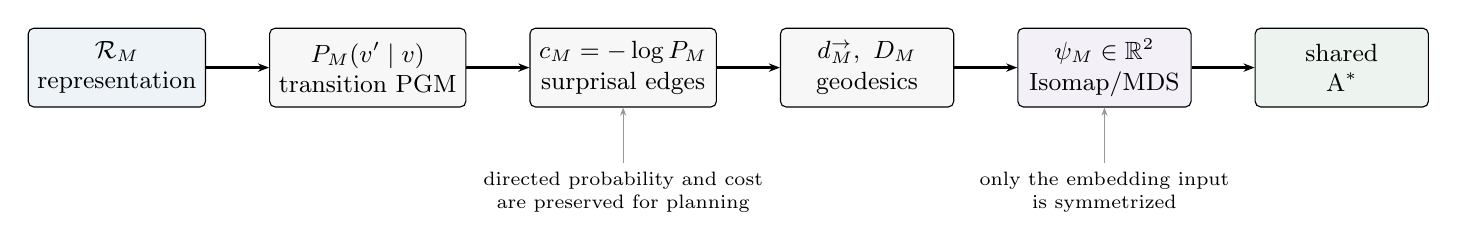
\begin{tikzpicture}[node distance=7mm and 8mm]
  \node[stage,fill=landmarkcol!8] (R) {$\mathcal R_M$\\representation};
  \node[stage,right=of R] (P) {$P_M(v'\mid v)$\\transition PGM};
  \node[stage,right=of P] (C) {$c_M=-\log P_M$\\surprisal edges};
  \node[stage,right=of C] (D) {$d_M^\to,\ D_M$\\geodesics};
  \node[stage,right=of D,fill=mapcol!8] (Psi) {$\psi_M\in\mathbb R^2$\\Isomap/MDS};
  \node[stage,right=of Psi,fill=goalcol!8] (A) {shared\\A$^\ast$};
  \draw[arrow] (R)--(P);
  \draw[arrow] (P)--(C);
  \draw[arrow] (C)--(D);
  \draw[arrow] (D)--(Psi);
  \draw[arrow] (Psi)--(A);
  \node[font=\scriptsize,align=center,below=7mm of C] (directed)
    {directed probability and cost\\are preserved for planning};
  \node[font=\scriptsize,align=center,below=7mm of Psi] (sym)
    {only the embedding input\\is symmetrized};
  \draw[-{Stealth[length=3pt]},black!40] (directed.north)--(C.south);
  \draw[-{Stealth[length=3pt]},black!40] (sym.north)--(Psi.south);
\end{tikzpicture}
\caption{The shared probability-to-planning pipeline. Action grammar probabilities and
landmark CPDs enter through different representations but produce the same downstream
objects.}
\label{fig:pipeline}
\end{figure}

\section{One \texorpdfstring{A$^\ast$}{A-star} algorithm for every representation}
\label{sec:astar}

A$^\ast$ searches the original directed graph
$(\mathcal V_M,\mathcal E_M,c_M)$, not the symmetrized embedding graph. For a current node
$v$ and goal $s_\star$, its evaluation function is
\begin{equation}
f_M(v)=g_M(v)+h_M(v,s_\star),
\label{eq:astar-score}
\end{equation}
where $g_M(v)$ is accumulated directed surprisal cost. To obtain a valid heuristic from
the learned coordinates, define
\begin{equation}
\alpha_M
=
\min_{\substack{(u,v)\in\mathcal E_M:\\
\|\psi_M(u)-\psi_M(v)\|_2>0}}
\frac{c_M(u,v)}
{\|\psi_M(u)-\psi_M(v)\|_2},
\qquad
h_M(v,s_\star)
=
\alpha_M\|\psi_M(v)-\psi_M(s_\star)\|_2.
\label{eq:scaled-heuristic}
\end{equation}
If every supported edge has zero embedded length, set $\alpha_M=0$. Deterministic
probability-one edges can likewise make $\alpha_M=0$; in that degenerate case A$^\ast$
reduces to Dijkstra's algorithm while remaining correct.

For every directed edge $(u,v)$, Euclidean triangle inequality and
\eqref{eq:scaled-heuristic} give
\begin{align}
h_M(u,s_\star)
&\le
\alpha_M\|\psi_M(u)-\psi_M(v)\|_2+h_M(v,s_\star)\nonumber\\
&\le
c_M(u,v)+h_M(v,s_\star).
\label{eq:consistency}
\end{align}
Thus $h_M$ is consistent and therefore admissible. A$^\ast$ returns the same
minimum-surprisal path as Dijkstra's algorithm when allowed to terminate normally.

\begin{center}
\fbox{\begin{minipage}{0.92\textwidth}
\textbf{Shared A$^\ast$ planner.}
Initialize $g(s_0)=0$ and an open priority queue ordered by
$f(v)=g(v)+h(v,s_\star)$. Repeatedly remove the node with smallest $f$, terminate when
$s_\star$ is removed, and relax every supported directed edge using cost $c_M(u,v)$.
Reopen a node if a lower $g$ is found. Search budget, queue tie-breaking, and termination
rules are fixed across agent families. Only $P_M$, hence $c_M$ and $\psi_M$, changes.
\end{minipage}}
\end{center}

\begin{figure}[htbp]
\centering
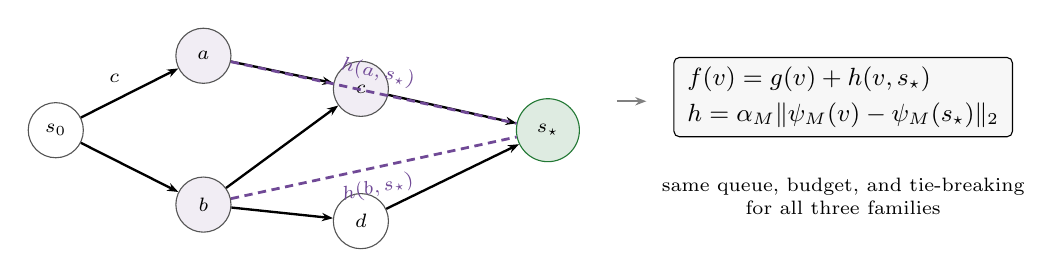
\begin{tikzpicture}[x=1.25cm,y=1.05cm]
  \node[state] (s) at (0,0) {$s_0$};
  \node[state,fill=mapcol!10] (a) at (1.5,0.9) {$a$};
  \node[state,fill=mapcol!10] (b) at (1.5,-0.9) {$b$};
  \node[state,fill=mapcol!10] (c) at (3.1,0.5) {$c$};
  \node[state] (d) at (3.1,-1.1) {$d$};
  \node[goal] (g) at (5.0,0) {$s_\star$};
  \draw[arrow] (s)--node[above left,font=\scriptsize] {$c$}(a);
  \draw[arrow] (s)--(b);
  \draw[arrow] (a)--(c);
  \draw[arrow] (b)--(c);
  \draw[arrow] (b)--(d);
  \draw[arrow] (c)--(g);
  \draw[arrow] (d)--(g);
  \draw[densely dashed,mapcol,line width=1pt] (a)--(g)
    node[midway,above,sloped,font=\scriptsize] {$h(a,s_\star)$};
  \draw[densely dashed,mapcol,line width=1pt] (b)--(g)
    node[midway,below,sloped,font=\scriptsize] {$h(b,s_\star)$};
  \node[stage,align=left,minimum width=43mm] at (8.0,0.4)
    {$f(v)=g(v)+h(v,s_\star)$\\[2pt]
     $h=\alpha_M\|\psi_M(v)-\psi_M(s_\star)\|_2$};
  \node[font=\scriptsize,align=center] at (8.0,-0.8)
    {same queue, budget, and tie-breaking\\for all three families};
  \draw[arrow,black!50] (5.7,0.35)--(6.0,0.35);
\end{tikzpicture}
\caption{A$^\ast$ uses directed surprisal for accumulated path cost and scaled manifold
distance for estimated remaining cost. The embedding guides expansion order without
changing the optimum.}
\label{fig:astar}
\end{figure}

\section{Worked \texorpdfstring{$3\times3$}{3 by 3} landmark example}
\label{sec:example}

Let $\mathcal S=\{1,\ldots,9\}$,
\[
\mathcal L=\{1,5,9\},
\qquad
\mathcal U=\{2,3,4,6,7,8\}.
\]
For each landmark $\ell$, assign probability $0.30$ to each of the other two landmarks
and probability $1/15$ to each non-landmark. Set $p(\ell\mid\ell)=0$. Each landmark row
therefore sums to
\[
2(0.30)+6(1/15)=1.
\]
For non-landmarks, define rows over landmarks $(1,5,9)$ as follows:
\begin{center}
\begin{tabular}{c@{\qquad}ccc}
\toprule
$u$ & $p(1\mid u)$ & $p(5\mid u)$ & $p(9\mid u)$\\
\midrule
2 & .60 & .25 & .15\\
3 & .55 & .30 & .15\\
4 & .30 & .55 & .15\\
6 & .15 & .55 & .30\\
7 & .15 & .30 & .55\\
8 & .15 & .25 & .60\\
\bottomrule
\end{tabular}
\end{center}
Every non-landmark row sums to one and every non-landmark-to-non-landmark entry is zero.
The strongest peripheral detour between two landmarks has probability
\[
\max_u p(u\mid\ell)p(\ell'\mid u)
=
\frac{1}{15}(0.60)
=
0.04
<
0.30
=
p(\ell'\mid\ell),
\]
so the core constraint holds with a wide margin. For example,
\[
d_{\mathrm L}^\to(1,5)=-\log(0.30)\approx1.204,
\]
whereas the best two-edge peripheral detour between those landmarks costs at least
$-\log(0.04)\approx3.219$. A path between two non-landmarks must have the form
\[
u
\longrightarrow
\ell_i
\longrightarrow\cdots\longrightarrow
\ell_j
\longrightarrow
u',
\]
so the landmark core necessarily mediates peripheral planning. The transition graph is
strongly connected, all directed geodesics are finite, and applying
\eqref{eq:symmetric-distance}--\eqref{eq:embedding} yields a finite two-dimensional map in
which $\{1,5,9\}$ forms the compact central core relative to the non-landmark periphery.
For this numerical kernel, normalized two-dimensional MDS stress is approximately $0.418$.
The embedding is therefore a lossy coordinate chart, as expected for this core--periphery
graph; quantitative representational comparisons should use the full $D_{\mathrm L}$,
while A$^\ast$ remains valid because its heuristic is scaled by
\eqref{eq:scaled-heuristic}.

\section{What Analysis 7 does not model}

This document stops at representation and planning. It does not introduce a
change-point process, segment identities, trajectory emissions, a complete-data
likelihood, structural EM, or model-family recovery. Those objects concern how an analyst
infers $\mathcal R_M$ and its parameters from behavior and belong in Analysis 8. Keeping
that inference machinery separate prevents the agent's cognitive map from being defined
by the analyst's segmentation algorithm.

\section{Summary}

All three agents are now comparable at one interface. Primitive action probabilities,
action-grammar probabilities, or landmark CPDs induce a row-stochastic transition kernel
$P_M$. Negative log probability turns that kernel into an additive directed geometry;
geodesic symmetrization and Isomap/classical MDS produce $\psi_M$; and a globally scaled
Euclidean heuristic lets the same A$^\ast$ planner search every representation without
sacrificing optimality. The landmark hypothesis is specifically the core--periphery PGM
in \eqref{eq:landmark-kernel}: non-landmarks cannot transition directly to one another, so
plans between them are organized through a tightly connected landmark core.

\end{document}
